% !TeX root = ../tesi.tex
% !TeX encoding = UTF-8
% !TeX spellcheck = it_IT

\chapter{Associazione con l'engagement}
\label{chap:associazione-engagement}

In questo capitolo rispondo alla domanda di ricerca: quanto contribuiscono il contenuto delle regioni sospette e le caratteristiche visive alla classificazione dell'engagement, rispetto al solo punteggio TruFor? Presento il campione e il protocollo comune (Sezione~\ref{sec:associazione-impostazione}), poi esamino il solo punteggio globale di TruFor (Sezione~\ref{sec:associazione-trufor}), le caratteristiche visive (Sezione~\ref{sec:associazione-visive}) e il testo (Sezione~\ref{sec:associazione-testo}). Descrivo la ricerca degli iperparametri tramite grid search (Sezione~\ref{sec:associazione-grid-search}) e confronto i blocchi informativi (Sezione~\ref{sec:associazione-confronto-blocchi}). Concludo con l'interpretazione delle previsioni sulle parole (Sezione~\ref{sec:associazione-spiegazioni}). Per ogni confronto affianco procedura, risultati e interpretazione.

\section{Campione, modelli e protocollo di valutazione}
\label{sec:associazione-impostazione}

Uso le informazioni prodotte dai rami dei Capitoli~\ref{chap:localizzazione-descrizione} e~\ref{chap:caratteristiche-visive}: il punteggio globale TruFor $t_i$, il testo delle regioni sospette e le 19 caratteristiche dell'immagine intera. Le associo al punteggio continuo di engagement $c_i$ e alla risposta binaria $y_i$, definiti nella Sottosezione~\ref{subsec:dataset-engagement} e nell'Equazione~\ref{eq:dataset-target}. La classe 1 indica prestazioni superiori alle aspettative dell'account; la classe 0 indica prestazioni inferiori.

Indico con $n$ il numero di osservazioni dell'analisi. Uso i campioni distinti nella Sottosezione~\ref{subsec:dataset-statistiche}, mantenendo allineati risposta e predittori. La Tabella~\ref{tab:associazione-campione} incrocia le classi di engagement con la disponibilità della descrizione testuale. Anche le osservazioni con \texttt{nomask} partecipano alla classificazione: la loro codifica è descritta nella Sottosezione~\ref{subsec:associazione-testo-preparazione}.

\begin{table}[htbp]
    \centering\small
    \caption{Disponibilità della descrizione per classe di engagement nel campione di classificazione. Conteggi da \texttt{results/dataset\_filtered.csv}, dopo l'esclusione dei casi con $|c_i|\leq0{,}5$.}
    \label{tab:associazione-campione}
    \begin{tabular}{@{}lrrr@{}}
        \toprule
        Classe & Descrizione testuale & \texttt{nomask} & Totale \\
        \midrule
        1: sopra le aspettative & 440 & 143 & 583 \\
        0: sotto le aspettative & 446 & 166 & 612 \\
        \midrule
        Totale & 886 & 309 & 1.195 \\
        \bottomrule
    \end{tabular}
\end{table}

Uso SciPy per le correlazioni~\cite{2020SciPy-NMeth}, statsmodels per OLS e GLM~\cite{josef_perktold_2024_10984387} e scikit-learn~\cite{scikit-learn} per vettorizzazione, PCA e regressione logistica.

Avvio le analisi con \path{scripts/classification_home.py}. Lo script condivide le funzioni di preparazione dei dati fra i moduli di classificazione. Riporto i valori dei report finali in \path{scripts/temp/}.

\subsection{Modello binomiale e significato dei coefficienti}
\label{subsec:associazione-glm}

Per la risposta binaria uso un GLM binomiale con collegamento logit, corrispondente alla regressione logistica introdotta nella Sottosezione~\ref{subsec:background-glm}. Con il vettore di predittori $\mathbf{u}_i$ scrivo:
\begin{equation}
    \log\frac{p_i}{1-p_i}=\beta_0+\sum_j\beta_j u_{ij},
    \qquad p_i=\Pr(y_i=1\mid\mathbf{u}_i).
    \label{eq:classificazione-logit}
\end{equation}

Indico con $\beta_0$ l'intercetta e con $\beta_j$ il coefficiente del predittore $u_{ij}$. Il rapporto $p_i/(1-p_i)$ esprime le \emph{odds}, ossia il rapporto tra la probabilità che l'evento si verifichi e la probabilità che non si verifichi. A parità degli altri predittori, un incremento $\Delta$ della variabile $j$ moltiplica le odds per $\exp(\beta_j\Delta)$. L'\emph{odds ratio} $\exp(\beta_j)$ riguarda un incremento unitario. Per un peso TF-IDF non equivale all'aggiunta di una parola, che modifica anche la normalizzazione della riga.

Distinguo due finalità. Per la predizione uso la logistica con \emph{penalità L2}, detta anche \emph{ridge}: aggiungo alla funzione da minimizzare un termine proporzionale alla somma dei quadrati dei coefficienti. In scikit-learn il parametro $C$ è l'inverso dell'intensità della regolarizzazione: valori più piccoli impongono una penalizzazione maggiore. Per esaminare coefficienti, intervalli di confidenza e test uso il GLM stimato per massima verosimiglianza~\cite{68aee965-a8a0-3e72-9f89-8d89ae91a62b}. Quando questo fit non converge, ricorro alla regolarizzazione senza attribuire p-value ai coefficienti ottenuti.

Nei test sui coefficienti l'ipotesi nulla è $H_0:\beta_j=0$. Interpreto i valori di $p$~\cite{10.1007/11744078_23} secondo la Sottosezione~\ref{subsec:background-p-value}.

\subsection{Adattamento e prestazioni in validazione}
\label{subsec:materiali-metriche-classificazione}

Misuro l'adattamento sui dati di stima con lo pseudo-$R^2$ di McFadden:
\begin{equation}
    R^2_{\mathrm{McF}}=1-\frac{\ell_{\mathrm{modello}}}{\ell_{\mathrm{nullo}}},
    \label{eq:materiali-mcfadden}
\end{equation}
dove $\ell$ indica la log-verosimiglianza e il modello nullo contiene la sola intercetta. Quest'ultimo assegna a tutti i casi la prevalenza della classe 1. Un valore maggiore segnala un migliore adattamento rispetto al riferimento; non esprime una quota di varianza spiegata~\cite{mcfadden1972conditional}.

Per la \emph{validazione incrociata}, CV (Cross-Validation), suddivido il campione in cinque parti disgiunte. A turno, escludo una parte dalla stima dei coefficienti e uso il modello stimato sulle altre quattro per prevedere le probabilità delle osservazioni escluse. Riunisco queste probabilità per calcolare le metriche.

Per le probabilità $\widehat p_i^{\mathrm{CV}}$ così ottenute, definisco la perdita logaritmica media e l'indice di confronto con il riferimento nullo:
\begin{equation}
    L_{\mathrm{CV}}=-\frac{1}{n}\sum_i
    \left[y_i\log\widehat p_i^{\mathrm{CV}}+
    (1-y_i)\log(1-\widehat p_i^{\mathrm{CV}})\right],
    \qquad Q_{\mathrm{CV}}=1-\frac{L_{\mathrm{CV}}}{L_0}.
    \label{eq:classificazione-cv}
\end{equation}
Il riferimento $L_0$ usa la prevalenza $\bar y$ dell'intero campione. I report chiamano $Q_{\mathrm{CV}}$ \emph{McFadden pseudo-R2} o \emph{CV R2}: ne riprende la forma, ma usa previsioni da modelli stimati su partizioni diverse. Lo distinguo quindi da $R^2_{\mathrm{McF}}$ in-sample. Un valore negativo indica una perdita maggiore del riferimento; un valore positivo indica una perdita minore.

Per la logistica assegno la classe 1 quando la probabilità prevista è almeno $0{,}5$. Calcolo l'accuratezza come quota di classificazioni corrette e la confronto con la baseline che assegna sempre la classe 0, pari al $51{,}2\%$. L'AUC misura la capacità di ordinare un caso positivo sopra uno negativo, assegnando metà peso alle parità; il riferimento senza discriminazione è $0{,}5$.

\subsection{Partizioni e limiti del protocollo}
\label{subsec:metodi-classificazione-validazione}

Le partizioni sono \emph{stratificate} quando mantengono approssimativamente le proporzioni delle classi del campione. La \emph{grid search} confronta tutte le combinazioni di valori prefissati degli \emph{iperparametri}, cioè delle impostazioni scelte prima della stima dei coefficienti. La Tabella~\ref{tab:associazione-validazione} distingue le suddivisioni effettivamente implementate.

\begin{table}[htbp]
    \centering\small
    \caption{Protocolli di validazione dei modelli di classificazione. Le trasformazioni dei predittori precedono la suddivisione.}
    \label{tab:associazione-validazione}
    \begin{tabular}{@{}p{0.25\linewidth}p{0.42\linewidth}p{0.22\linewidth}@{}}
        \toprule
        Analisi & Suddivisione & Metriche \\
        \midrule
        Logistica L2 & 5 partizioni stratificate, senza mescolamento & Accuratezza, AUC, $Q_{\mathrm{CV}}$ \\
        \addlinespace
        Confronto dei GLM & 5 partizioni non stratificate, mescolate con seme 42; comuni ai quattro modelli & $Q_{\mathrm{CV}}$ \\
        \addlinespace
        Grid search & Stessa procedura a 5 partizioni mescolate, seme 42 & $Q_{\mathrm{CV}}$ per configurazione \\
        \bottomrule
    \end{tabular}
\end{table}

Nel protocollo implementato apprendo vocabolario, pesi IDF, PCA e standardizzazione visiva sull'intero campione prima della suddivisione. Anche la prevalenza del riferimento nullo usa tutte le etichette. Le osservazioni di validazione sono escluse dalla stima dei coefficienti, ma partecipano alla preparazione dei dati. Questa scelta può introdurre ottimismo nella valutazione. Inoltre, la diversa suddivisione di logistica e GLM impedisce di attribuire le differenze tra i loro report alla sola regolarizzazione. Le partizioni non separano account o periodi e non misurano la generalizzazione a nuovi contesti.

\newpage
\section{Il solo punteggio TruFor come riferimento}
\label{sec:associazione-trufor}

Studio prima quanto il solo punteggio globale $t_i$ sia associato all'engagement. Uso $c_i$ per correlazioni e regressione lineare, e $y_i$ per il GLM binomiale. Questo confronto fornisce il riferimento per valutare le informazioni aggiunte dalla pipeline. La Tabella~\ref{tab:metodi-trufor-analisi} collega ciascuna analisi alla sua implementazione.

\begin{table}[htbp]
    \centering
    \small
    \caption{Funzioni di \texttt{scripts/trufor.py} e chiamate di libreria usate per le analisi sul solo punteggio TruFor.}
    \label{tab:metodi-trufor-analisi}
    \begin{tabular}{@{}>{\raggedright\arraybackslash}p{0.23\linewidth}>{\raggedright\arraybackslash}p{0.22\linewidth}>{\raggedright\arraybackslash}p{0.46\linewidth}@{}}
        \toprule
        Analisi & Funzione nello script & Chiamata di libreria \\
        \midrule
        Correlazione di Pearson & \texttt{correlation} & \path{scipy.stats.pearsonr} \\
        \addlinespace
        Correlazione di Spearman & \texttt{correlation} & \path{scipy.stats.spearmanr} \\
        \addlinespace
        Regressione lineare & \texttt{regression} & \path{statsmodels.api.OLS} \\
        \addlinespace
        GLM binomiale & \texttt{glm} & \path{statsmodels.api.GLM} con \path{statsmodels.api.families.Binomial} \\
        \bottomrule
    \end{tabular}
\end{table}

\subsection{Correlazioni tra i punteggi}
\label{subsec:associazione-trufor-correlazioni}

Indico con $(v_i,w_i)$ le coppie di valori osservati e con $\bar v$, $\bar w$ le loro medie. Formalizzo il coefficiente di Pearson, introdotto nella Sottosezione~\ref{subsec:background-pearson}:
\begin{equation}
    r(v,w)=\frac{\sum_i(v_i-\bar v)(w_i-\bar w)}
    {\sqrt{\sum_i(v_i-\bar v)^2\sum_i(w_i-\bar w)^2}}.
    \label{eq:materiali-pearson}
\end{equation}
Il segno indica la direzione e il valore assoluto la forza dell'associazione. Il coefficiente di Pearson varia in $[-1,1]$ ed è sensibile alle osservazioni estreme~\cite{10.1098/rspl.1895.0041}. Per il coefficiente di Spearman, introdotto nella Sottosezione~\ref{subsec:background-spearman}, applico Pearson ai ranghi, con rango medio in caso di parità:
\begin{equation}
    \rho_s(v,w)=r\!\left(\operatorname{rank}(v),\operatorname{rank}(w)\right).
    \label{eq:materiali-spearman}
\end{equation}
Anche Spearman varia in $[-1,1]$. Entrambi i coefficienti sono indefiniti per una variabile costante e non stabiliscono rapporti causali~\cite{ca468a70-0be4-389a-b0b9-5dd1ff52b33f}.

Calcolo i due coefficienti tra $t_i$ e $c_i$ sulle 1.211 osservazioni, con test bilaterali dell'ipotesi di correlazione nulla. I valori della Tabella~\ref{tab:risultati-trufor-correlazioni} sono positivi e vicini allo zero: l'associazione lineare e quella monotona risultano deboli.

\begin{table}[htbp]
    \centering
    \small
    \caption{Correlazioni tra il punteggio globale di TruFor e lo score di engagement sulle 1.211 osservazioni. Valori riportati nel report di correlazione \texttt{trufor\_crowdtangle\_correlation.txt}.}
    \label{tab:risultati-trufor-correlazioni}
    \begin{tabular}{@{}lrr@{}}
        \toprule
        Correlazione & Coefficiente & Valore di $p$ \\
        \midrule
        Pearson & $0{,}055$ & $0{,}05760$ \\
        Spearman & $0{,}043$ & $0{,}1368$ \\
        \bottomrule
    \end{tabular}
\end{table}

\subsection{Regressione lineare sul punteggio continuo}
\label{subsec:associazione-trufor-ols}

Stimo una regressione lineare con intercetta sulle 1.211 osservazioni:
\begin{equation}
    c_i=\beta_0+\beta_1t_i+\varepsilon_i,
    \label{eq:materiali-ols}
\end{equation}
dove $\beta_0$ è l'intercetta, $\beta_1$ esprime la variazione media dello score di engagement associata a un incremento unitario di TruFor e $\varepsilon_i$ è il termine di errore dell'osservazione $i$. Il metodo dei minimi quadrati ordinari, OLS (Ordinary Least Squares), stima i parametri minimizzando gli scarti quadratici~\cite{James2013}:
\begin{equation}
    (\widehat\beta_0,\widehat\beta_1)=\operatorname*{arg\,min}_{\beta_0,\beta_1}
    \sum_i[c_i-(\beta_0+\beta_1t_i)]^2.
    \label{eq:materiali-minimi-quadrati}
\end{equation}
Con $\widehat c_i=\widehat\beta_0+\widehat\beta_1t_i$ misuro l'adattamento mediante:
\begin{equation}
    R^2=1-\frac{\sum_i(c_i-\widehat c_i)^2}{\sum_i(c_i-\bar c)^2}.
    \label{eq:materiali-r-quadro}
\end{equation}
In questo modello con intercetta, valutato sui dati di stima, $R^2$ esprime la quota di variabilità spiegata. Lo distinguo dallo pseudo-$R^2$ del GLM e dalla valutazione su osservazioni escluse dalla stima.

Il modello spiega circa lo $0{,}3\%$ della variabilità nel campione (Tabella~\ref{tab:risultati-trufor-lineare}). La pendenza è positiva, ma il suo intervallo di confidenza comprende lo zero. Questi risultati confermano il contributo limitato del punteggio alla descrizione dell'engagement continuo.

\begin{table}[htbp]
    \centering\small
    \caption{Regressione OLS di $c_i$ su TruFor, con intercetta. Fonte: \texttt{trufor\_crowdtangle\_regression.txt}.}
    \label{tab:risultati-trufor-lineare}
    \begin{tabular}{@{}lr@{}}
        \toprule
        Quantità & Valore \\
        \midrule
        Numero di osservazioni & 1.211 \\
        Coefficiente associato a TruFor & $4{,}8879$ \\
        Intervallo di confidenza al $95\%$ & $[-0{,}158;\,9{,}934]$ \\
        Valore di $p$ & $0{,}058$ \\
        $R^2$ sui dati di stima & $0{,}003$ \\
        \bottomrule
    \end{tabular}
\end{table}

\subsection{GLM per le due classi di engagement}
\label{subsec:risultati-trufor-glm}

Dopo l'esclusione dell'intervallo centrale, stimo il GLM~\cite{68aee965-a8a0-3e72-9f89-8d89ae91a62b} con TruFor come unico predittore e con intercetta:
\begin{equation}
    \log\frac{p_i}{1-p_i}=\beta_0+\beta_1t_i.
    \label{eq:materiali-glm}
\end{equation}
Verifico la convergenza e calcolo l'adattamento sul campione di 1.195 osservazioni.

Ottengo $R^2_{\mathrm{McF}}=0{,}0009$ (Tabella~\ref{tab:risultati-trufor-glm}). Il coefficiente è positivo, con intervallo di confidenza che comprende lo zero. Nel protocollo comune ai quattro GLM ottengo inoltre $Q_{\mathrm{CV}}=-0{,}0060$: la perdita in validazione supera quella del riferimento a probabilità costante.

\begin{table}[htbp]
    \centering
    \small
    \caption{GLM binomiale con il punteggio globale di TruFor e l'intercetta. Lo pseudo-$R^2$ riguarda i dati usati per la stima. Fonte: report del GLM \texttt{trufor\_crowdtangle\_glm.txt}.}
    \label{tab:risultati-trufor-glm}
    \begin{tabular}{@{}lr@{}}
        \toprule
        Quantità & Valore \\
        \midrule
        Numero di osservazioni & 1.195 \\
        Coefficiente associato a TruFor & $0{,}2731$ \\
        Intervallo di confidenza al $95\%$ del coefficiente & $[-0{,}160;\,0{,}706]$ \\
        Valore di $p$ del coefficiente & $0{,}217$ \\
        Pseudo-$R^2$ di McFadden & $0{,}0009$ \\
        \bottomrule
    \end{tabular}
\end{table}

\subsection{Interpretazione del riferimento}
\label{subsec:risultati-trufor-riferimento}

Il solo TruFor mostra un'associazione debole con l'engagement e una capacità predittiva limitata nel campione. Il punteggio riassume gli indizi del rilevatore: non misura l'intenzione comunicativa o l'esposizione degli utenti al post. Queste analisi riguardano l'engagement e restano distinte dalla valutazione forense del Capitolo~\ref{chap:localizzazione-descrizione}.

\section{Associazioni delle caratteristiche visive}
\label{sec:associazione-visive}

Uso le 19 caratteristiche dell'immagine intera, definite nel Capitolo~\ref{chap:caratteristiche-visive}, per due confronti. Esamino prima le associazioni di ciascuna misura con engagement e TruFor. Valuto poi il blocco visivo nel GLM, insieme al punteggio TruFor.

\subsection{Protocollo delle correlazioni}
\label{subsec:metodi-feature-correlazioni}

Ripeto il confronto con Pearson~\cite{10.1098/rspl.1895.0041} e Spearman~\cite{ca468a70-0be4-389a-b0b9-5dd1ff52b33f}, definiti nella Sottosezione~\ref{subsec:associazione-trufor-correlazioni}. Con ciascun metodo, per ogni caratteristica $j$ calcolo due correlazioni sulle osservazioni disponibili:
\begin{equation}
    a_j=\operatorname{corr}(f_{ij},c_i),
    \qquad
    b_j=\operatorname{corr}(f_{ij},t_i),
    \qquad j=1,\ldots,19.
    \label{eq:feature-correlazioni}
\end{equation}
Qui $c_i$ è il punteggio continuo di engagement e $t_i$ è il punteggio globale di TruFor. In questo passaggio conservo anche i punteggi di engagement nell'intervallo $[-0{,}5;\,0{,}5]$. Il calcolo esclude i valori mancanti separatamente per ogni coppia di variabili.

Nelle Figure~\ref{fig:risultati-feature-pearson} e~\ref{fig:risultati-feature-spearman} rappresento ciascuna caratteristica con il punto $(a_j,b_j)$ ottenuto rispettivamente con Pearson e Spearman. Ogni grafico contiene quindi 19 descrittori, ciascuno riassuntivo delle associazioni calcolate su tutte le immagini. Aggiungo la retta $b=a$, riferimento di uguaglianza dei coefficienti con segno, e una retta adattata ai punti con i minimi quadrati, usando $a_j$ come predittore e $b_j$ come risposta.

\bigskip\noindent
\begin{minipage}{\linewidth}
    \captionsetup{type=figure}
    \centering
    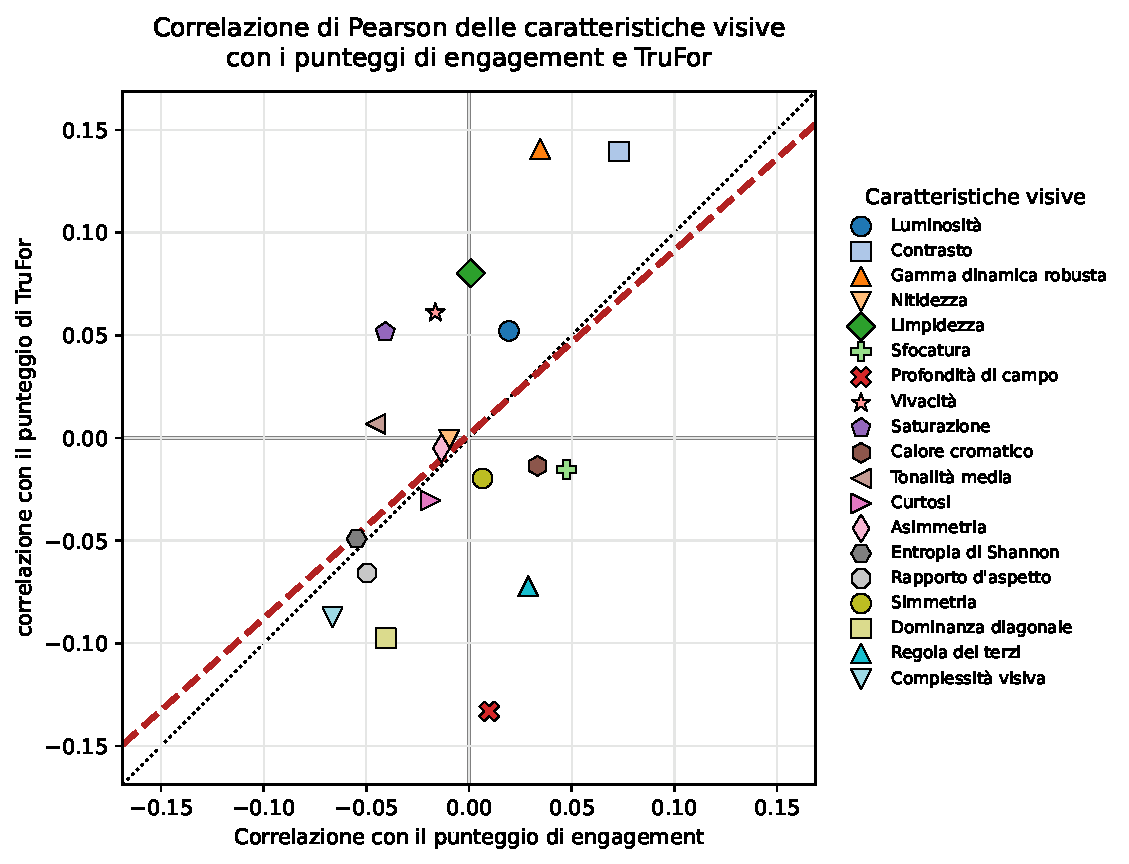
\includegraphics[width=0.8\linewidth]{caratteristiche_visive_pearson.pdf}
    \caption{Correlazioni di Pearson sulle 1.211 osservazioni. Ogni punto rappresenta una caratteristica. La retta nera puntinata indica $b=a$; quella rossa tratteggiata riassume i 19 punti. Fonte: \texttt{images\_features\_pearson.txt}.}
    \label{fig:risultati-feature-pearson}
    \par\medskip
    \captionsetup{type=figure}
    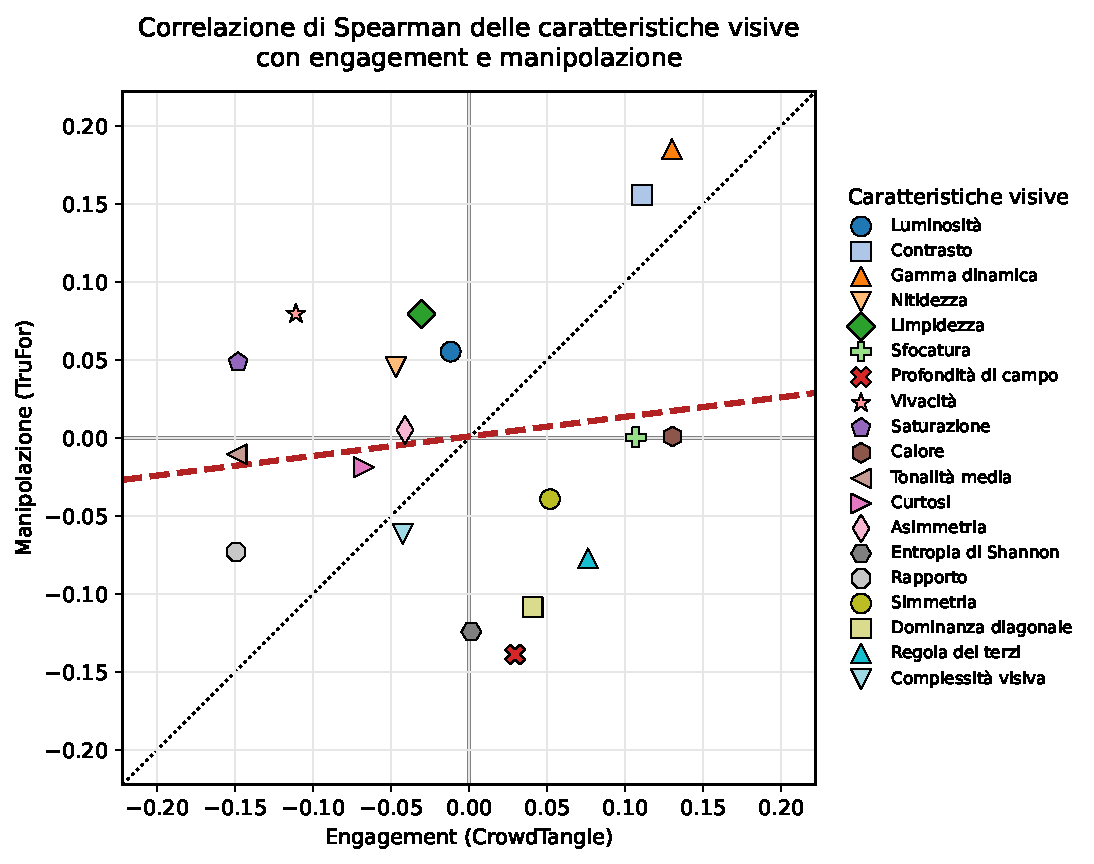
\includegraphics[width=0.8\linewidth]{caratteristiche_visive_spearman.pdf}
    \caption{Correlazioni di Spearman sulle 1.211 osservazioni. Ogni punto rappresenta una caratteristica. La retta nera puntinata indica $b=a$; quella rossa tratteggiata riassume i 19 punti. Fonte: \texttt{images\_features\_spearman.txt}.}
    \label{fig:risultati-feature-spearman}
\end{minipage}
\par\bigskip

Le caratteristiche possono essere correlate tra loro e le due coordinate derivano dallo stesso campione: la retta riassume il confronto tra descrittori e non costituisce un modello di previsione dell'engagement delle immagini. Escludo dal grafico le caratteristiche con correlazioni non definite, come avviene per una colonna costante.

Per Pearson uso \path{images_features_pearson.txt}, per Spearman uso \path{images_features_spearman.txt}. Ogni report ordina le caratteristiche per $|b_j|$ decrescente. Lo script produce coefficienti descrittivi senza valori di $p$ o intervalli di confidenza.

\subsection{Risultati delle correlazioni e lettura congiunta}
\label{subsec:associazione-visive-correlazioni}

Dispongo di tutte le variabili per le 1.211 osservazioni. La Tabella~\ref{tab:risultati-feature-correlazioni} mostra associazioni contenute con entrambi i metodi. Per l'engagement, Spearman evidenzia diverse associazioni più marcate rispetto a Pearson. Le correlazioni con TruFor mantengono più spesso segno e valori simili.

\begin{table}[htbp]
    \centering
    \small
    \caption{Correlazioni di Pearson e Spearman sulle stesse 1.211 osservazioni. Fonti: \texttt{images\_features\_pearson.txt} e \texttt{images\_features\_spearman.txt}.}
    \label{tab:risultati-feature-correlazioni}
    \begin{tabular}{@{}lrrrr@{}}
        \toprule
        & \multicolumn{2}{c}{Pearson ($r$)} & \multicolumn{2}{c}{Spearman ($\rho_s$)} \\
        \cmidrule(lr){2-3}\cmidrule(l){4-5}
        Caratteristica & Engagement & TruFor & Engagement & TruFor \\
        \midrule
        Luminosità & $+0{,}0194$ & $+0{,}0521$ & $-0{,}0118$ & $+0{,}0553$ \\
        Contrasto & $+0{,}0729$ & $+0{,}1394$ & $+0{,}1108$ & $+0{,}1559$ \\
        Gamma dinamica robusta & $+0{,}0347$ & $+0{,}1406$ & $+0{,}1300$ & $+0{,}1851$ \\
        Nitidezza & $-0{,}0097$ & $-0{,}0009$ & $-0{,}0468$ & $+0{,}0453$ \\
        Limpidezza & $+0{,}0008$ & $+0{,}0802$ & $-0{,}0305$ & $+0{,}0794$ \\
        Sfocatura & $+0{,}0474$ & $-0{,}0154$ & $+0{,}1069$ & $+0{,}0004$ \\
        Profondità di campo & $+0{,}0098$ & $-0{,}1331$ & $+0{,}0295$ & $-0{,}1388$ \\
        Vivacità & $-0{,}0164$ & $+0{,}0610$ & $-0{,}1110$ & $+0{,}0796$ \\
        Saturazione & $-0{,}0408$ & $+0{,}0516$ & $-0{,}1481$ & $+0{,}0486$ \\
        Calore & $+0{,}0334$ & $-0{,}0136$ & $+0{,}1304$ & $+0{,}0009$ \\
        Tonalità media & $-0{,}0455$ & $+0{,}0069$ & $-0{,}1490$ & $-0{,}0104$ \\
        Curtosi & $-0{,}0187$ & $-0{,}0304$ & $-0{,}0675$ & $-0{,}0188$ \\
        Asimmetria & $-0{,}0134$ & $-0{,}0050$ & $-0{,}0410$ & $+0{,}0051$ \\
        Entropia di Shannon & $-0{,}0547$ & $-0{,}0492$ & $+0{,}0014$ & $-0{,}1242$ \\
        Rapporto d'aspetto & $-0{,}0496$ & $-0{,}0658$ & $-0{,}1493$ & $-0{,}0730$ \\
        Simmetria & $+0{,}0065$ & $-0{,}0197$ & $+0{,}0519$ & $-0{,}0392$ \\
        Dominanza diagonale & $-0{,}0406$ & $-0{,}0976$ & $+0{,}0407$ & $-0{,}1084$ \\
        Regola dei terzi & $+0{,}0288$ & $-0{,}0722$ & $+0{,}0763$ & $-0{,}0772$ \\
        Complessità visiva & $-0{,}0665$ & $-0{,}0874$ & $-0{,}0425$ & $-0{,}0617$ \\
        \bottomrule
    \end{tabular}
\end{table}

Le Figure~\ref{fig:risultati-feature-pearson} e~\ref{fig:risultati-feature-spearman} rappresentano le stesse caratteristiche: la coordinata orizzontale indica la correlazione con l'engagement, quella verticale la correlazione con TruFor. Mantengo simboli e colori, adattando i limiti degli assi a ciascun metodo. La retta rossa riassume le posizioni dei 19 descrittori: presenta pendenza positiva con Pearson ed è più vicina all'orizzontale con Spearman.

Le associazioni con l'engagement restano inferiori a $0{,}15$ in valore assoluto. Il contrasto è correlato positivamente con entrambi gli indicatori; la saturazione è correlata negativamente con l'engagement e positivamente con TruFor. Per rapporto d'aspetto, tonalità media e saturazione, Spearman rileva associazioni più marcate con l'engagement rispetto a Pearson. Si tratta di confronti descrittivi, una caratteristica alla volta.

\subsection{Il blocco visivo aggiunto a TruFor}
\label{subsec:associazione-visive-glm}

Stimo un GLM non penalizzato con TruFor e le 19 caratteristiche standardizzate: sottraggo la media e divido per la deviazione standard calcolate sul campione. Ogni coefficiente visivo esprime così la variazione dei log-odds per un incremento di una deviazione standard, a parità degli altri predittori. La Tabella~\ref{tab:associazione-visive-coefficienti} riporta i coefficienti, gli intervalli al $95\%$ e i p-value non corretti dei test di Wald. Uso il test di Wald per verificare, per ciascun coefficiente, l’ipotesi nulla che sia uguale a zero~\cite{60455556-c6b2-37bb-9077-b6ce7e1443d8}.

Rispetto al solo TruFor, lo pseudo-$R^2_{\mathrm{McF}}$ passa da $0{,}0009$ a $0{,}0624$ e $Q_{\mathrm{CV}}$ da $-0{,}0060$ a $0{,}0278$. Il blocco visivo migliora quindi entrambi gli indici nel protocollo adottato. Confronto questo incremento con quello del testo nella Sezione~\ref{sec:associazione-confronto-blocchi}.

Applico Benjamini--Hochberg ai 19 p-value visivi, escludendo intercetta e TruFor dalla famiglia di verifiche~\cite{10.1111/j.2517-6161.1995.tb02031.x}. Considero significativo un coefficiente quando il valore corretto $p_{\mathrm{BH}}$, indicato con \texttt{q} nel report, è inferiore a $0{,}05$. Solo \texttt{aspect\_ratio} risulta significativo dopo la correzione: $\beta=-0{,}2177$ per deviazione standard e $p_{\mathrm{BH}}=0{,}0219<0{,}05$. La correzione riguarda il modello TruFor e visive, non il modello completo.

Il rapporto larghezza/altezza presenta un'associazione negativa condizionata agli altri predittori inclusi. Account, piattaforma e periodo rimangono fuori dal modello: non ricavo quindi una prescrizione sul formato che aumenterebbe l'engagement. I coefficienti delle altre caratteristiche, incluso il calore cromatico, non risultano significativi dopo la correzione; questo esito non prova l'assenza di una loro associazione nella popolazione.

\begin{table}[htbp]
    \centering\small
    \caption{Coefficienti delle 19 caratteristiche nel GLM TruFor e visive. Gli intervalli sono al $95\%$ e i p-value sono non corretti. Dopo Benjamini--Hochberg~\cite{10.1111/j.2517-6161.1995.tb02031.x} soltanto il rapporto d'aspetto risulta significativo, con $p_{\mathrm{BH}}=0{,}0219<0{,}05$. Fonte: \texttt{classification\_visual\_text.txt}.}
    \label{tab:associazione-visive-coefficienti}
    \begin{tabular}{@{}lrrr@{}}
        \toprule
        Caratteristica & $\beta$ per dev.\ std. & Intervallo & $p$ \\
        \midrule
        Rapporto d'aspetto & $-0{,}2177$ & $[-0{,}349;\,-0{,}086]$ & $0{,}001$ \\
        Luminosità & $-0{,}2857$ & $[-0{,}606;\,0{,}035]$ & $0{,}081$ \\
        Contrasto & $0{,}2246$ & $[-0{,}024;\,0{,}474]$ & $0{,}077$ \\
        Gamma dinamica robusta & $-0{,}0217$ & $[-0{,}215;\,0{,}171]$ & $0{,}825$ \\
        Nitidezza & $0{,}0034$ & $[-0{,}224;\,0{,}231]$ & $0{,}977$ \\
        Limpidezza & $-0{,}0584$ & $[-0{,}372;\,0{,}256]$ & $0{,}716$ \\
        Sfocatura & $0{,}1471$ & $[-0{,}018;\,0{,}313]$ & $0{,}082$ \\
        Profondità di campo & $-0{,}0425$ & $[-0{,}183;\,0{,}098]$ & $0{,}553$ \\
        Vivacità & $-0{,}0119$ & $[-0{,}258;\,0{,}234]$ & $0{,}925$ \\
        Saturazione & $-0{,}2719$ & $[-0{,}527;\,-0{,}017]$ & $0{,}037$ \\
        Calore & $0{,}2072$ & $[0{,}058;\,0{,}357]$ & $0{,}007$ \\
        Tonalità media & $-0{,}0551$ & $[-0{,}217;\,0{,}107]$ & $0{,}505$ \\
        Curtosi & $-0{,}0332$ & $[-0{,}272;\,0{,}206]$ & $0{,}785$ \\
        Asimmetria & $-0{,}1498$ & $[-0{,}467;\,0{,}167]$ & $0{,}355$ \\
        Entropia di Shannon & $-0{,}0419$ & $[-0{,}273;\,0{,}189]$ & $0{,}723$ \\
        Simmetria & $0{,}1798$ & $[0{,}033;\,0{,}326]$ & $0{,}016$ \\
        Dominanza diagonale & $0{,}0103$ & $[-0{,}166;\,0{,}186]$ & $0{,}909$ \\
        Regola dei terzi & $0{,}1184$ & $[-0{,}026;\,0{,}263]$ & $0{,}109$ \\
        Complessità visiva & $0{,}1344$ & $[-0{,}066;\,0{,}335]$ & $0{,}189$ \\
        \bottomrule
    \end{tabular}
\end{table}

\newpage
\section{Contributo del testo delle regioni sospette}
\label{sec:associazione-testo}

Valuto due rappresentazioni dello stesso testo: i pesi delle parole e le componenti PCA. In entrambi i casi includo il punteggio TruFor. Distinguo le prestazioni della logistica regolarizzata dalla stima dei GLM, perché rispondono a finalità diverse.

\subsection{Preparazione e rappresentazioni testuali}
\label{subsec:associazione-testo-preparazione}

Rimuovo le stop word italiane e inglesi, normalizzate come le descrizioni, e \texttt{nomask}. Estraggo unigrammi di almeno due caratteri. Conservo i termini presenti in almeno cinque descrizioni e in non più del $40\%$ del campione; fra quelli ammessi mantengo al massimo i cento più frequenti.

Indico con $n_{ij}$ le occorrenze della parola $j$ nella descrizione $i$ e con $d_j$ il numero di descrizioni che la contengono. Uso la variante TF-IDF con regolarizzazione delle frequenze documentali~\cite{scikit-learn}:
\begin{equation}
    a_{ij}=n_{ij}\left[1+\log\left(\frac{1+n}{1+d_j}\right)\right],
    \qquad x_{ij}=\frac{a_{ij}}{\sqrt{\sum_k a_{ik}^2}}.
    \label{eq:classificazione-tfidf}
\end{equation}
Normalizzo ogni riga alla norma euclidea unitaria. Se nessun termine appartiene al vocabolario, mantengo un vettore nullo. Questo accade anche per \texttt{nomask}: la codifica unisce quindi assenza di descrizione e assenza di parole conservate dai filtri.

Per la seconda rappresentazione centro le colonne TF-IDF, senza standardizzarle, e applico la PCA~\cite{jolliffe2016principal}. Fisso la varianza da conservare al $90\%$ e ottengo 61 componenti. Una riga TF-IDF nulla può avere coordinate PCA diverse da zero per effetto della centratura. TruFor rimane separato e non entra nella PCA.

Per i GLM regolarizzati indico con $\alpha$ l'intensità della penalizzazione. La \emph{penalità L1}, detta \emph{lasso}, usa la somma dei valori assoluti dei coefficienti; \emph{elastic net} combina L1 e L2. La quota L1 regola questa combinazione: 0 corrisponde a ridge, 1 a lasso e i valori intermedi a elastic net. Riassumo la configurazione nella Tabella~\ref{tab:classificazione-parametri}.

\begin{table}[htbp]
    \centering
    \small
    \caption{Configurazione della classificazione. I parametri condivisi provengono da \texttt{scripts/config.py}; la logistica usa le impostazioni predefinite di scikit-learn~\cite{scikit-learn} salvo il limite di iterazioni.}
    \label{tab:classificazione-parametri}
    \begin{tabular}{@{}lr@{}}
        \toprule
        Parametro & Valore \\
        \midrule
        Intervallo escluso per l'engagement & $[-0{,}5;\,0{,}5]$ \\
        Vocabolario massimo & 100 unigrammi \\
        Frequenza documentale minima / massima & 5 / $40\%$ \\
        Varianza da conservare con PCA & $90\%$ \\
        Logistica: penalità / parametro $C$ & L2 / 1 \\
        Logistica: massimo di iterazioni & 1.000 \\
        GLM: penalità di ripiego $\alpha$ / quota L1 & $0{,}0007$ / 0 \\
        Partizioni di validazione & 5 \\
        Permutazioni per predittore & 30 \\
        Casi spiegati con LIME & 5 \\
        \bottomrule
    \end{tabular}
\end{table}

\subsection{Prestazioni della regressione logistica}
\label{subsec:risultati-classificazione-logistica}

Con \path{classification_logistic_regression.py} addestro la logistica L2, con $C=1$ e massimo 1.000 iterazioni. Uso \texttt{cross\_val\_predict} con le cinque partizioni stratificate della Sottosezione~\ref{subsec:metodi-classificazione-validazione}. Per gli odds ratio riaddestro invece il modello sull'intero campione.

La Tabella~\ref{tab:risultati-classificazione-logistica} confronta cento parole TF-IDF e 61 componenti PCA, sempre con TruFor. Ottengo un'accuratezza del $59{,}4\%$, circa 8,2 punti percentuali sopra la baseline del $51{,}2\%$. Il TF-IDF presenta AUC e $Q_{\mathrm{CV}}$ leggermente maggiori. La riduzione dei predittori conserva quindi una prestazione vicina a quella della rappresentazione lessicale.

\begin{table}[htbp]
    \centering
    \small
    \caption{Regressione logistica L2 sulle due rappresentazioni testuali, entrambe con TruFor. Metriche sulle previsioni riunite delle cinque partizioni; baseline di maggioranza: $51{,}2\%$. Fonte: \texttt{classification\_logistic\_regression.txt}.}
    \label{tab:risultati-classificazione-logistica}
    \begin{tabular}{@{}lrrrr@{}}
        \toprule
        Testo & Predittori & Accuratezza & AUC & $Q_{\mathrm{CV}}$ \\
        \midrule
        TF-IDF & 101 & $59{,}4\%$ & $0{,}644$ & $0{,}0613$ \\
        TF-IDF con PCA & 62 & $59{,}4\%$ & $0{,}638$ & $0{,}0582$ \\
        \bottomrule
    \end{tabular}
\end{table}

Entrambe le configurazioni classificano correttamente 710 casi (Tabella~\ref{tab:associazione-confusioni}). Restano 485 errori: le rappresentazioni mostrano una capacità predittiva modesta. I report non forniscono intervalli d'incertezza per le differenze fra le prestazioni.

\begin{table}[htbp]
    \centering\small
    \caption{Conteggi delle matrici di confusione in validazione, con classe positiva 1 e soglia $0{,}5$. TP (True Positives) e TN (True Negatives) indicano rispettivamente i veri positivi e i veri negativi; FP (False Positives) e FN (False Negatives) indicano i falsi positivi e i falsi negativi. Fonte: \texttt{classification\_logistic\_regression.txt}.}
    \label{tab:associazione-confusioni}
    \begin{tabular}{@{}lrrrrr@{}}
        \toprule
        Testo, con TruFor & TP & TN & FP & FN & \shortstack{Previsioni\\corrette} \\
        \midrule
        TF-IDF & 293 & 417 & 195 & 290 & 710 \\
        TF-IDF con PCA & 297 & 413 & 199 & 286 & 710 \\
        \bottomrule
    \end{tabular}
\end{table}

\subsection{Stima dei GLM sulle rappresentazioni testuali}
\label{subsec:associazione-testo-glm}

Con \path{classification_glm.py} stimo i GLM per massima verosimiglianza tramite \emph{IRLS (Iteratively Reweighted Least Squares)}, cioè minimi quadrati iterativamente ripesati. Includo l'intercetta e controllo convergenza e finitezza della log-verosimiglianza. Se il controllo fallisce, uso ridge con $\alpha=0{,}0007$, senza errori standard o p-value. La regolarizzazione stabilizza la stima in presenza di problemi come la separazione; il solo fallimento numerico non ne costituisce una diagnosi completa~\cite{10.1093/biomet/71.1.1}.

Sul TF-IDF il GLM non penalizzato non supera il controllo di convergenza e ricorro al fit ridge (Tabella~\ref{tab:associazione-glm-testo}). Sulle componenti PCA il GLM converge. In quest'ultimo modello, il coefficiente di TruFor è $0{,}4998$, con intervallo al $95\%$ $[-0{,}033;\,1{,}033]$ e $p=0{,}066$. I coefficienti delle componenti combinano più parole: i loro test non identificano singoli termini associati all'engagement.

\begin{table}[htbp]
    \centering\small
    \caption{GLM sulle due rappresentazioni testuali, con TruFor. L'indice riguarda i dati di stima. Fonte: \texttt{classification\_glm.txt}.}
    \label{tab:associazione-glm-testo}
    \begin{tabular}{@{}lrrl@{}}
        \toprule
        Testo & Predittori & $R^2_{\mathrm{McF}}$ & Stima utilizzata \\
        \midrule
        TF-IDF & 101 & $0{,}1383$ & Ridge, senza p-value \\
        TF-IDF con PCA & 62 & $0{,}1369$ & Non penalizzata \\
        \bottomrule
    \end{tabular}
\end{table}

\newpage
\subsection{Interpretazione del contributo testuale}
\label{subsec:associazione-testo-interpretazione}

Il GLM con testo PCA raggiunge $Q_{\mathrm{CV}}=0{,}0234$, rispetto a $-0{,}0060$ del solo TruFor, nelle stesse partizioni. Il risultato sostiene l'utilità di studiare il contenuto selezionato, entro i limiti del protocollo. Non dimostra che descrivere le regioni sospette sia meglio che descrivere l'immagine intera: manca un classificatore basato su descrizioni dell'immagine intera ottenute con gli stessi strumenti. Il contributo osservato appartiene alla rappresentazione prodotta dalla pipeline nel suo insieme.

\section{Ricerca esplorativa degli iperparametri}
\label{sec:associazione-grid-search}

Applico la grid search introdotta nella Sottosezione~\ref{subsec:metodi-classificazione-validazione} tramite la modalità \texttt{--grid-search} di \path{classification_glm.py} per esplorare i filtri documentali e la penalità del GLM sul TF-IDF, sempre insieme a TruFor. Il parametro $\alpha$ controlla l'intensità della penalità; la quota L1 ne distingue la componente lasso da quella ridge. La ricerca non usa la PCA e non seleziona il parametro $C$ della logistica L2. Considero le combinazioni della Tabella~\ref{tab:associazione-grid-parametri}, mantenendo il limite di cento parole e lo stesso campione di 1.195 osservazioni.

\begin{table}[htbp]
    \centering\small
    \caption{Griglia esplorata, da \texttt{classification\_glm\_grid\_search.txt}. La quota L1 distingue ridge (0), elastic net ($0{,}5$) e lasso (1).}
    \label{tab:associazione-grid-parametri}
    \begin{tabular}{@{}lp{0.62\linewidth}@{}}
        \toprule
        Parametro & Valori \\
        \midrule
        \texttt{min\_df} & 2, 5, 10 descrizioni \\
        \texttt{max\_df} & $0{,}4$; $0{,}5$; $0{,}6$; $0{,}7$; $0{,}8$ \\
        Penalità $\alpha$ & 0; $0{,}0001$; $0{,}0005$; $0{,}0007$; $0{,}001$; $0{,}005$; $0{,}01$ \\
        Quota L1 & 0; $0{,}5$; 1, solo per $\alpha>0$ \\
        Totale & $3\times5\times(1+6\times3)=285$ configurazioni \\
        \bottomrule
    \end{tabular}
\end{table}

Per ogni coppia di filtri ricostruisco il TF-IDF sull'intero campione. Valuto poi le penalità con cinque partizioni non stratificate, mescolate con seme 42, e ordino le configurazioni per $Q_{\mathrm{CV}}$. Per $\alpha=0$ eseguo una sola valutazione, perché la quota L1 non modifica il modello. Controllo inoltre se il GLM non penalizzato converge su tutto il campione per ciascuna coppia di filtri.

Ottengo un punteggio per le 270 configurazioni penalizzate; le 15 non penalizzate non superano la valutazione nelle partizioni. Inoltre, nessuna delle 15 coppie di filtri produce un GLM non penalizzato convergente sull'intero campione. Il report non individua quindi una configurazione che conservi i p-value del fit non penalizzato.

Il massimo è $Q_{\mathrm{CV}}=0{,}0647$, con \texttt{min\_df}=5, \texttt{max\_df}=$0{,}4$ e ridge con $\alpha=0{,}0007$ (Tabella~\ref{tab:associazione-grid-risultati}). Questi valori coincidono con la configurazione adottata. La ricerca documenta la scelta dei parametri, ma il massimo è selezionato sullo stesso campione e sulle stesse partizioni usate per confrontare le configurazioni. Non lo considero una stima indipendente della prestazione: servirebbe una valutazione esterna alla selezione degli iperparametri.

\begin{table}[htbp]
    \centering\small
    \caption{Migliore configurazione riportata per ciascuna famiglia di penalità. Tutte conservano cento parole. Le altre quattro soglie \texttt{max\_df} danno lo stesso punteggio arrotondato per ciascuna riga. Fonte: \texttt{classification\_glm\_grid\_search.txt}.}
    \label{tab:associazione-grid-risultati}
    \begin{tabular}{@{}lrrrrr@{}}
        \toprule
        Penalità & \texttt{min\_df} & \texttt{max\_df} & $\alpha$ & Quota L1 & $Q_{\mathrm{CV}}$ \\
        \midrule
        Ridge & 5 & $0{,}4$ & $0{,}0007$ & 0 & $0{,}0647$ \\
        Elastic net & 5 & $0{,}4$ & $0{,}0007$ & $0{,}5$ & $0{,}0596$ \\
        Lasso & 2 & $0{,}4$ & $0{,}001$ & 1 & $0{,}0556$ \\
        \bottomrule
    \end{tabular}
\end{table}

\section{Confronto dei blocchi informativi}
\label{sec:associazione-confronto-blocchi}

Con \path{classification_visual_text.py} confronto quattro GLM non penalizzati sulle stesse 1.195 osservazioni e con le stesse partizioni: TruFor; TruFor e testo PCA; TruFor e caratteristiche visive; tutti i predittori insieme. I modelli includono l'intercetta, esclusa dal conteggio dei predittori. Il testo descrive le regioni sospette, mentre le 19 caratteristiche standardizzate descrivono l'immagine intera.

La Tabella~\ref{tab:risultati-confronto-blocchi} e la Figura~\ref{fig:classificazione-confronto-modelli} mostrano un miglioramento rispetto al solo TruFor quando aggiungo separatamente testo o caratteristiche visive. Il modello con le caratteristiche visive ottiene il maggiore $Q_{\mathrm{CV}}$, ma la differenza rispetto al testo è contenuta e non dispone di un intervallo d'incertezza.

\begin{table}[htbp]
    \centering
    \small
    \caption{Confronto dei blocchi sul medesimo campione di 1.195 osservazioni. Distinguo lo pseudo-$R^2$ in-sample dall'indice $Q_{\mathrm{CV}}$ calcolato con cinque partizioni comuni ai quattro GLM. Fonte: \texttt{classification\_visual\_text.txt}.}
    \label{tab:risultati-confronto-blocchi}
    \begin{tabular}{@{}lrrr@{}}
        \toprule
        Predittori & Numero & $R^2_{\mathrm{McF}}$ & $Q_{\mathrm{CV}}$ \\
        \midrule
        TruFor & 1 & $0{,}0009$ & $-0{,}0060$ \\
        TruFor e testo & 62 & $0{,}1369$ & $0{,}0234$ \\
        TruFor e visive & 20 & $0{,}0624$ & $0{,}0278$ \\
        TruFor, testo e visive & 81 & $0{,}1605$ & $0{,}0128$ \\
        \bottomrule
    \end{tabular}
\end{table}

\begin{figure}[htbp]
    \centering
    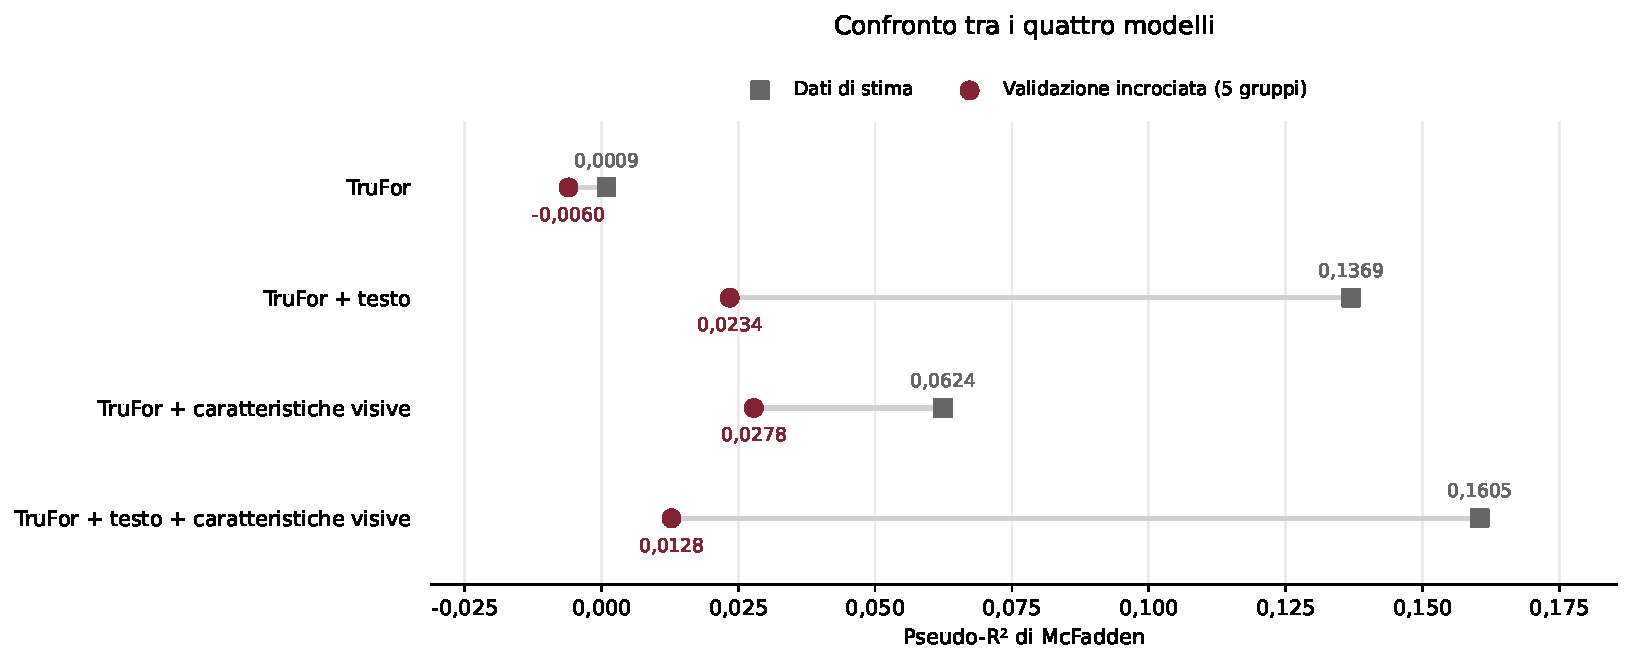
\includegraphics[width=\linewidth]{classificazione_confronto_modelli.pdf}
    \caption{Adattamento e validazione dei quattro GLM. I quadrati indicano $R^2_{\mathrm{McF}}$ sui dati di stima; i cerchi indicano $Q_{\mathrm{CV}}$ in validazione incrociata. Valori più alti indicano un risultato migliore; zero corrisponde al riferimento basato sulla frequenza delle classi e valori negativi indicano un risultato peggiore del riferimento. La validazione riguarda la stima dei coefficienti del modello: TF-IDF, PCA e standardizzazione sono stimati sull'intero campione. Fonte: \texttt{classification\_visual\_text.txt}.}
    \label{fig:classificazione-confronto-modelli}
\end{figure}

\newpage
Il modello completo raggiunge il maggiore adattamento in-sample, $0{,}1605$, ma $Q_{\mathrm{CV}}$ scende a $0{,}0128$. Aggiungere le caratteristiche visive al testo migliora quindi il fit sui dati di stima senza migliorare la prestazione nel protocollo adottato. Per rispondere anche alla domanda sul contributo aggiuntivo delle descrizioni, confronto il modello completo con quello che comprende già TruFor e le caratteristiche visive: aggiungendo il testo, $Q_{\mathrm{CV}}$ passa da $0{,}0278$ a $0{,}0128$. Nel confronto osservato il testo non migliora quindi questo riferimento più informativo, pur migliorando quello basato sul solo TruFor. Un maggiore numero di coefficienti può rendere la stima più sensibile al campione. Anche una sovrapposizione fra informazioni visive e testuali è possibile, ma il risultato non dimostra che i due blocchi siano ridondanti.

Confronto inoltre le coppie di \emph{modelli annidati}: in questi confronti ottengo il modello ridotto ponendo a zero i coefficienti dei predittori aggiunti nel modello esteso. Uso la \emph{devianza} $D=2(\ell_{\mathrm{saturo}}-\ell_{\mathrm{modello}})$, che confronta la log-verosimiglianza del modello con quella del \emph{modello saturo}, capace di riprodurre esattamente ogni osservazione. La statistica del \emph{test del rapporto di verosimiglianza} è $\Lambda=D_{\mathrm{ridotto}}-D_{\mathrm{esteso}}$. Sotto l'ipotesi nulla e le condizioni di regolarità uso il riferimento asintotico $\chi^2$, con gradi di libertà pari al numero dei parametri aggiunti. Confronto ciascun modello intermedio con TruFor e il completo con TruFor e testo. I due modelli intermedi non sono annidati fra loro.

I test della Tabella~\ref{tab:associazione-rapporti-verosimiglianza} riguardano i coefficienti aggiunti sotto le ipotesi del GLM. Il risultato del modello completo rende concreta la distinzione: un test significativo accompagna un peggioramento in validazione. La significatività statistica non garantisce un vantaggio predittivo su nuovi dati.

\begin{table}[htbp]
    \centering\small
    \caption{Test del rapporto di verosimiglianza tra GLM annidati. I due valori di $p$ arrotondati a zero nel report sono indicati con $p<0{,}0001$. Fonte: \texttt{classification\_visual\_text.txt}.}
    \label{tab:associazione-rapporti-verosimiglianza}
    \begin{tabular}{@{}lrrr@{}}
        \toprule
        Estensione del modello & $\Lambda$ & Gradi di libertà & $p$ \\
        \midrule
        TruFor $\rightarrow$ TruFor e testo & $225{,}2$ & 61 & $<0{,}0001$ \\
        TruFor $\rightarrow$ TruFor e visive & $101{,}8$ & 19 & $<0{,}0001$ \\
        TruFor e testo $\rightarrow$ completo & $38{,}9$ & 19 & $0{,}0045$ \\
        \bottomrule
    \end{tabular}
\end{table}

Rispetto alla domanda di ricerca, osservo un contributo predittivo modesto delle rappresentazioni arricchite. Il testo e le caratteristiche visive aggiunti separatamente migliorano il riferimento TruFor. Il confronto con il modello che include già le caratteristiche visive non mostra invece un vantaggio predittivo aggiuntivo delle descrizioni. Questa conclusione riguarda il campione e il protocollo adottati, con preparazione dei predittori prima della suddivisione; non dimostra l'assenza di informazione utile nel testo in altri campioni o con altre rappresentazioni.

\section{Interpretazione delle previsioni sulle parole}
\label{sec:associazione-spiegazioni}

Con \path{classification_lime_shap.py} riaddestro la logistica su TruFor e sulle cento colonne TF-IDF dell'intero campione. Ispeziono il modello attraverso il report \path{classification_explanations.txt}. Le misure riguardano le osservazioni usate per stimarlo e non costituiscono una nuova valutazione predittiva.

\subsection{Protocollo delle spiegazioni}
\label{subsec:metodi-classificazione-spiegazioni}

Calcolo l'importanza per permutazione~\cite{JMLR:v20:18-760} come calo dell'AUC sul campione di stima. Ripeto il rimescolamento trenta volte per predittore, con seme 42. Riporto media e deviazione standard: quest'ultima descrive le permutazioni a modello fisso, non l'incertezza dovuta a nuovi campioni. Il criterio del report ``media maggiore di due deviazioni standard'' è descrittivo e non sostituisce un p-value.

Per SHAP~\cite{NIPS2017_8a20a862} uso il \emph{mascheramento indipendente} delle variabili tabulari: i valori delle variabili temporaneamente escluse vengono sostituiti con quelli del campione di riferimento, senza condizionarli ai valori delle variabili mantenute. L'operazione riguarda le colonne TruFor e TF-IDF, non i pixel dell'immagine; uso tutte le osservazioni come riferimento. In questa configurazione il contributo della variabile $j$ al predittore lineare è $\phi_{ij}=\beta_j(u_{ij}-\bar u_j)$, espresso nei log-odds. Ordino le variabili tramite la media $n^{-1}\sum_i|\phi_{ij}|$ e ricavo la direzione dal segno del coefficiente logistico. La media dei contributi con segno sullo stesso riferimento è invece nulla.

Per LIME uso la variante tabulare senza discretizzare le variabili continue, con seme 42. Con le impostazioni predefinite, genero le perturbazioni campionando indipendentemente i valori TF-IDF e TruFor da distribuzioni normali con media e deviazione standard stimate sull'intero campione. Adatto una regressione ridge alle probabilità della classe 1 prodotte dal classificatore per questi dati. Assegno alle perturbazioni pesi che diminuiscono esponenzialmente con il quadrato della distanza euclidea dall'osservazione da spiegare, calcolata sulle variabili standardizzate: i punti più vicini incidono quindi maggiormente sul surrogato locale~\cite{ribeiro2016whyitrustyou}. Seleziono cinque osservazioni a posizioni equidistanti nell'ordinamento delle probabilità previste. I coefficienti del surrogato possono riguardare anche termini assenti dalla descrizione: non rappresentano automaticamente contributi additivi alla singola previsione.

\subsection{Coefficienti, frequenza e importanza globale}
\label{subsec:risultati-spiegazioni-globali}

La Figura~\ref{fig:classificazione-parole} affianca tre quantità: il coefficiente logistico, la quota di descrizioni contenenti una parola e la media dei suoi valori SHAP assoluti. Quest'ultima determina l'area delle bolle. La frequenza è mostrata su scala logaritmica. Un coefficiente di ampiezza elevata può riguardare una parola rara: la lettura congiunta evita di confondere l'ampiezza del coefficiente con l'importanza media nel campione.

La Figura~\ref{fig:classificazione-parole-barre} riporta le otto parole con maggiore media $|\mathrm{SHAP}|$ per ciascun segno del coefficiente. I valori sono espressi nei log-odds, non in punti percentuali di probabilità.

\newpage
\begin{figure}[htbp]
    \centering
    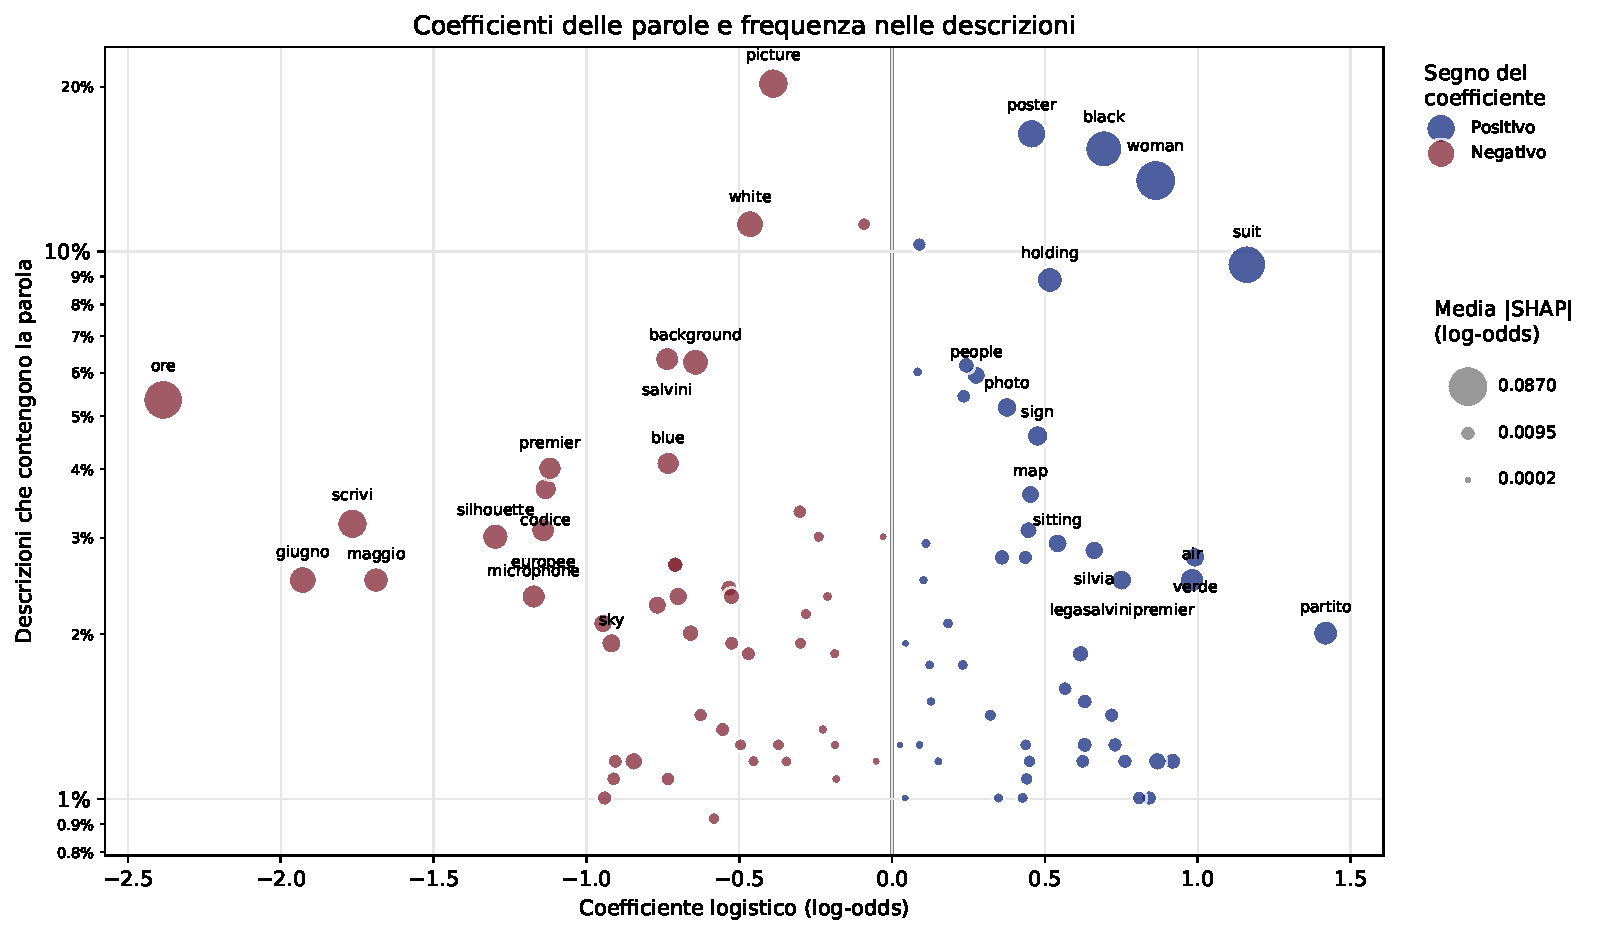
\includegraphics[width=\linewidth]{classificazione_parole.pdf}
    \caption{Coefficienti e frequenza delle parole nella logistica stimata sull'intero campione a fini interpretativi. L'area delle bolle indica la media $|\mathrm{SHAP}|$, prodotto tra $|\beta|$ e scarto assoluto medio dei valori TF-IDF: non è una misura indipendente. La distanza da zero non indica significatività; i p-value non sono disponibili perché il GLM sul TF-IDF grezzo non converge. I segni descrivono la previsione, non effetti causali.}
    \label{fig:classificazione-parole}
\end{figure}

\begin{figure}[htbp]
    \centering
    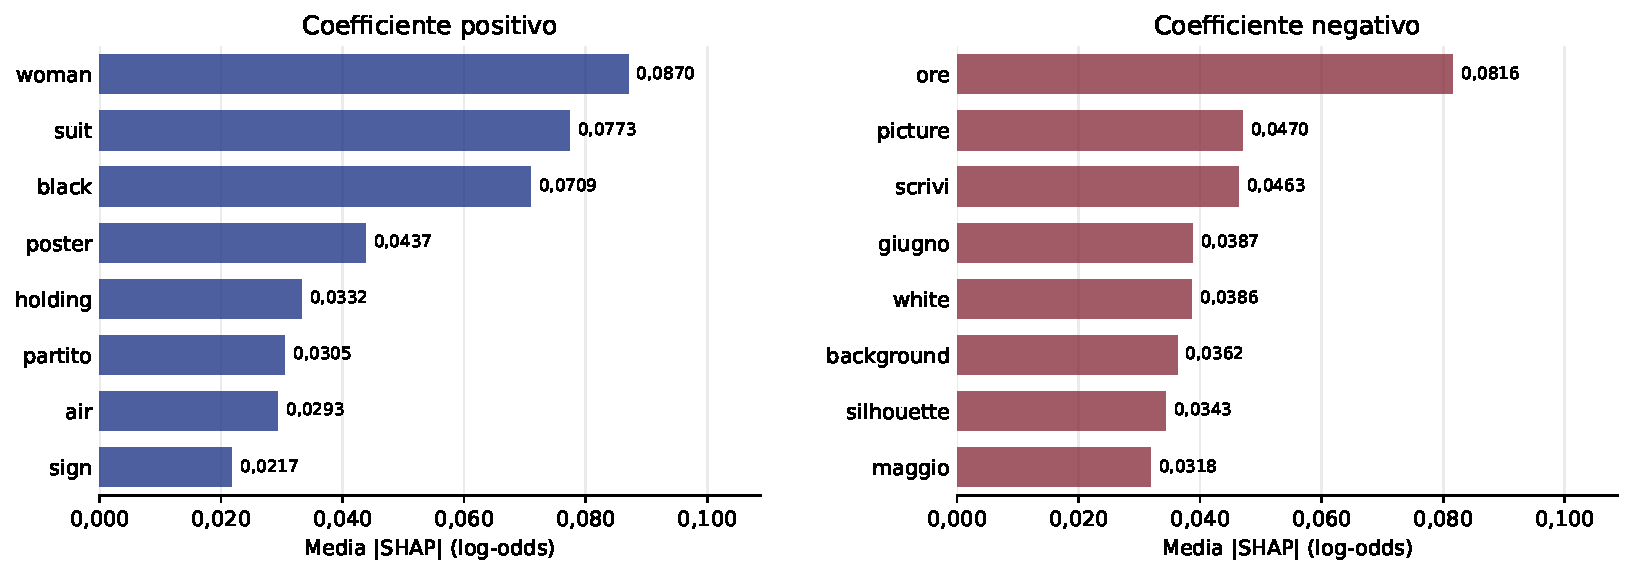
\includegraphics[width=\linewidth]{classificazione_parole_barre.pdf}
    \caption{Otto parole più importanti per media $|\mathrm{SHAP}|$~\cite{NIPS2017_8a20a862} sul campione di stima, divise per segno del coefficiente. I valori sono nei log-odds, non variazioni percentuali di probabilità, effetti causali o misure di significatività. Fonte: \texttt{classification\_explanations.txt}.}
    \label{fig:classificazione-parole-barre}
\end{figure}

Le due misure della Tabella~\ref{tab:associazione-parole-importanza} rispondono a domande diverse. SHAP scompone il predittore rispetto al riferimento; la permutazione valuta il cambiamento di una metrica quando rimescolo una colonna. La concordanza su alcuni termini non costituisce una conferma indipendente, perché entrambe usano lo stesso modello e campione.

\begin{table}[htbp]
    \centering\small
    \caption{Confronto fra SHAP~\cite{NIPS2017_8a20a862} e importanza per permutazione~\cite{JMLR:v20:18-760} per le due parole principali di ciascun segno nella Figura~\ref{fig:classificazione-parole-barre}. Dispersione su 30 permutazioni a modello fisso. Fonte: \texttt{classification\_explanations.txt}.}
    \label{tab:associazione-parole-importanza}
    \begin{tabular}{@{}lcrr@{}}
        \toprule
        Parola & Segno di $\beta$ & Media $|\mathrm{SHAP}|$ & Calo AUC: media $\pm$ dev.\ std. \\
        \midrule
        \texttt{woman} & $+$ & $0{,}0870$ & $0{,}0098\pm0{,}0042$ \\
        \texttt{suit} & $+$ & $0{,}0773$ & $0{,}0127\pm0{,}0043$ \\
        \texttt{ore} & $-$ & $0{,}0816$ & $0{,}0146\pm0{,}0059$ \\
        \texttt{picture} & $-$ & $0{,}0470$ & $0{,}0028\pm0{,}0036$ \\
        \bottomrule
    \end{tabular}
\end{table}

\newpage
Leggo le parole come indizi della rappresentazione automatica. Poiché il testo combina BLIP e OCR, termini relativi a persone, abbigliamento, date o manifesti possono riflettere il contenuto, gli autori dei post, gli errori di trascrizione o le caratteristiche del mascheramento. I coefficienti non permettono di separare queste spiegazioni.

\subsection{Due esempi locali con LIME}
\label{subsec:risultati-spiegazioni-locali}

Mostro i due casi estremi fra i cinque selezionati, identificati dai primi otto caratteri del nome del file. Il caso \texttt{c43374c2} ha $\widehat p=0{,}05$ e classe osservata 0: la descrizione menziona un uomo davanti a un televisore e contiene \texttt{ore} e \texttt{maggio}. Il caso \texttt{ca9681c6} ha $\widehat p=0{,}86$ e classe osservata 1: la stringa menziona un manifesto con un uomo e una donna e include \texttt{partito}.

Nella Tabella~\ref{tab:risultati-lime}, il peso di \texttt{ore} nel secondo caso descrive la sensibilità del surrogato alle perturbazioni, benché il termine sia assente.

\begin{table}[!htbp]
    \centering
    \small
    \caption{Coefficienti LIME~\cite{ribeiro2016whyitrustyou} dei due casi estremi sul campione di stima. ``Presente'' indica se il termine compare nella descrizione. Fonte: \texttt{classification\_explanations.txt}.}
    \label{tab:risultati-lime}
    \begin{tabular}{@{}llcr@{}}
        \toprule
        Caso & Termine & Presente & Coefficiente LIME \\
        \midrule
        \texttt{c43374c2} & \texttt{ore} & Sì & $-0{,}041$ \\
                           & \texttt{maggio} & Sì & $-0{,}018$ \\
                           & \texttt{woman} & No & $+0{,}033$ \\
        \addlinespace
        \texttt{ca9681c6} & \texttt{woman} & Sì & $+0{,}034$ \\
                           & \texttt{partito} & Sì & $+0{,}025$ \\
                           & \texttt{ore} & No & $-0{,}043$ \\
        \bottomrule
    \end{tabular}
\end{table}
